% For more information on compilation see: https://github.com/JuliaCon/JuliaConSubmission.jl
\documentclass{juliacon}
\setcounter{page}{1}
\usepackage{amsmath}
\usepackage{stackengine} % for decent underbars
\usepackage{subfig}
\usepackage{booktabs}
\usepackage{algorithm} % floating algorithm environment with algorithmic keywords
\usepackage{algpseudocode} % from algorithmicx
\usepackage{dcolumn}

\newcommand{\etal}{\textit{et al}.}
\newcommand{\ie}{\textit{i}.\textit{e}.}
\newcommand{\eg}{\textit{e}.\textit{g}.}
\newcommand\ubar[1]{\stackunder[1.2pt]{\(#1\)}{\rule{.8ex}{.075ex}}}

\newcolumntype{d}[1]{D{.}{.}{#1}}

\begin{document}

% **************GENERATED FILE, DO NOT EDIT**************

\title{Extending JumpProcesses.jl for fast point process simulation with time-varying intensities}

\author[1]{Guilherme Augusto Zagatti}
\author[3]{Samuel A. Isaacson}
\author[4]{Christopher Rackauckas}
\author[5]{Vasily Ilin}
\author[1, 2]{See-Kiong Ng}
\author[1, 2]{Stéphane Bressan}
\affil[1]{Institute of Data Science, National University of Singapore, Singapore}
\affil[2]{School of Computing, National University of Singapore, Singapore}
\affil[3]{Department of Mathematics and Statistics, Boston University}
\affil[4]{Computer Science and AI Laboratory (CSAIL), Massachusetts Institute of Technology}
\affil[5]{Department of Mathematics, University of Washington}

\keywords{Julia, Simulation, Jump process, Point process}

\hypersetup{
pdftitle = {Extending JumpProcesses.jl for fast point process simulation with time-varying intensities},
pdfsubject = {JuliaCon 2023 Proceedings},
pdfauthor = {Guilherme Augusto Zagatti, Samuel A. Isaacson, Christopher Rackauckas, Vasily Ilin, See-Kiong Ng, Stéphane Bressan},
pdfkeywords = {Julia, Simulation, Jump process, Point process},
}



\maketitle

\abstract{Point processes model the occurrence of a countable number of random points over some support. They can model diverse phenomena, such as chemical reactions, stock market transactions and social interactions. We show that \texttt{JumpProcesses.jl} is a fast, general-purpose library for simulating point processes. JumpProcesses.jl was first developed for simulating jump processes via stochastic simulation algorithms (SSAs) (including Doob’s method, Gillespie’s methods, and Kinetic Monte Carlo methods). Historically, jump processes have been developed in the context of dynamical systems to describe dynamics with discrete jumps.
In contrast, the development of point processes has been more focused on describing the occurrence of random events. In this paper, we bridge the gap between the treatment of point and jump process simulation. The algorithms previously included in \texttt{JumpProcesses.jl} can be mapped to three general methods developed in statistics for simulating evolutionary point processes. Our comparative exercise reveals that the library initially lacked an efficient algorithm for simulating processes with variable intensity rates. We, therefore, extended \texttt{JumpProcesses.jl} with a new simulation algorithm, \texttt{Coevolve}, that enables the rapid simulation of processes with locally-bounded variable intensity rates. It is now possible to efficiently simulate any point process on the real line with a non-negative, left-continuous, history-adapted and locally bounded intensity rate. This extension significantly improves the computational performance of \texttt{JumpProcesses.jl} when simulating such processes, enabling it to become one of the few readily available, fast, general-purpose libraries for simulating evolutionary point processes.}

\section{Introduction}

Methods for simulating the trajectory of evolutionary point processes can be split into exact and inexact methods. Exact methods describe the realization of each point in the process chronologically. Such methods are hard to scale for large populations where numerous events fire within a short period since every single point needs to be accounted for. Inexact methods trade accuracy for speed by simulating the total number of events in successive intervals. They are common in biochemistry, which often requires the simulation of chemical reactions in large systems.

Previously, most of the focus has been on either univariate processes with exotic intensities or large systems with conditionally constant intensities, but not on both. As such, there was no readily available general-purpose software for simulating compound point processes in large systems with time-dependent rates. We contribute a simulation algorithm \texttt{Coevolve} to \texttt{JumpProcesses.jl} for efficiently simulating such processes. The implemented algorithm improves the algorithm described in~\cite{farajtabar2017} from where it borrows its name. Among other improvements, our algorithm supports any process with locally bounded conditional intensity rates, adapts to intensity rates that do not change between jumps, and avoids the unnecessary re-computation of randomly generated numbers, as well as the computation of the intensity rate when its lower bound is available. The extension of \texttt{JumpProcesses.jl} significantly expands the type of models that can be simulated with the library, including compound inhomogeneous Poisson, Hawkes, and stress-release processes --- all described in~\cite{daley2003}. Since \texttt{JumpProcesses.jl} is a member of Julia's SciML organization, it also becomes easier to incorporate compound point processes with time-dependent rates in a wide variety of applications.

In this paper, we bridge the gap between simulation methods developed in statistics and biochemistry, which led us to the development of \texttt{Coevolve}. First, we briefly introduce evolutionary point processes. Next, since all simulation methods require a basic understanding of simulation methods for the Poisson homogeneous process, we first describe such methods. Then, we identify and discuss three general, exact methods. In the second part of this paper, we describe the algorithms in \texttt{JumpProcesses.jl} and how they relate to the literature. We highlight our contribution \texttt{Coevolve}, investigate the correctness of our implementation and provide performance benchmarks to demonstrate its value. The paper concludes by discussing potential improvements.

\section{The evolutionary point process} \label{sec:notation}

The evolutionary point process is a stochastic collection of marked points over a unidimensional support. They are exhaustively described in~\cite{daley2003}. The likelihood of any evolutionary point process is fully characterized by its conditional intensity and mark distribution :
\[ 
  \lambda^\ast (t) \equiv \lambda(t \mid H_{t^-} ) = \frac{\Pr(t \mid H_{t^-})}{1 - \Pr(t \mid H_{t^-})} \text{ and } f^\ast(k \mid t_n)
\]
Where \( H_{t^-} = \{ (t_n, k_n) \mid 0 \leq t_n \leq t \} \) denotes the internal history of the process up to but not including \( t \), and the superscript \( \ast \) denotes the conditoning of a function on the internal history. We can interpret the conditonal intensity as the likelihood of observing a point in the next infinitesimal unit of time, given that no point has occurred since the last observed point in \( H_{t^-} \).


\section{The homogeneous process} \label{sec:method-poisson}

A homogeneous process can be simulated using properties of the Poisson process, which allow us to describe two equivalent sampling procedures. The first procedure consists of drawing successive inter-arrival times. We know that the distance between any two points in a homogeneous process is distributed according to the exponential distribution --- see Theorem 7.2~\cite{last2017}. Given the homogeneous process with intensity \( \lambda \), then the distance \( \Delta t \) between two points is distributed according to \( \Delta t \sim \exp(1/\lambda) \). Draws from the exponential distribution can be performed by drawing from a uniform distribution in the interval \( [0, 1] \). If \( V \sim U[0, 1] \), then \( T = - ln(V) \, / \, \lambda \sim \exp(1) \). When a point process is homogeneous, the \textit{inverse} method of Subsection~\ref{subsec:sim-inverse} reduces to this approach. Thus, we defer the presentation of this Algorithm to the next section.

The second procedure uses the fact that Poisson processes can be represented as a mixed binomial process with a Poisson mixing distribution --- see Proposition 3.5~\cite{last2017}. In particular, the total number of points of a Poisson homogeneous process in \( [0, T) \) is distributed according to \( \mathcal{N} (T) \sim \operatorname{Poisson}( \lambda T ) \) and the location of each point within the region is distributed according to the uniform distribution \( t_n \sim U[0, T] \). 

% Tau leaping methods in Subsection~\ref{subsec:sim-tau} use a similar procedure to focus only on sampling the total number of points in successive intervals.

% Algorithm~\ref{algo:sim-mixed} lists the implementation of this approach.

% \begin{algorithm}[h]
% \begin{algorithmic}[1]
%   \Procedure{MixedBinomialMethod}{\( [0, T) \), \( \lambda \),}
%   \State initialize the history \( H_{T^-} \leftarrow \{ \} \)
%   \State draw the total number of points \( N \sim \operatorname{Poisson}( \lambda T ) \)
%   \For{\(n \leftarrow 1, N\)}
%       \State draw the location \( t_n \sim U[0, T] \)
%       \State update the history \( H_{T^-} \leftarrow H_{T^-} \cup (t_n) \)
%   \EndFor
%   \State \Return \( H_{T^-} \)
%   \EndProcedure
% \end{algorithmic}
% \caption{The mixed binomial method for simulating a homogeneous point process over a fixed duration of time \( [0, T) \).}
% \label{algo:sim-mixed}
% \end{algorithm}

\section{Exact simulation methods} \label{sec:method-exact}

\subsection{Inverse methods} \label{subsec:sim-inverse}

The \textit{inverse} method leverages Theorem 7.4.I~\cite{daley2003} which states that every simple point process~\footnote{A simple point process is a process in which the probability of observing more than one point in the same location is zero.} can be transformed to a homogeneous Poisson process with unit rate via the following formula:
\begin{equation} \label{eqn:inverse}
  \int_{t_{n-1}}^{t_n} \lambda^\ast \, (u) \, du = \Delta \tilde{t}_n \text{ , } \Delta \tilde{t}_n \sim \exp(1)
\end{equation}
The idea is to draw realizations from the unit rate Poisson process and solve Equation~\ref{eqn:inverse} above to obtain the desired point process. In Algorithm~\ref{algo:sim-inverse}, we adapt Algorithm 7.4~\cite{daley2003}. The advantage of using the inverse method is that it is easier to couple the point process with differential equations and solve the system with the same numerical integrator.


Whenever the conditional intensity is constant between two points, Equation~\ref{eqn:inverse} can be solved analytically. Let \( \lambda^\ast \, (t) = \lambda_{n-1} , \forall t_{n-1} \leq t < t_n \), then
\[
\begin{split}
  &\int_{t_{n-1}}^{t_n} \lambda^\ast \, (u) \, du = \Delta \tilde{t}_{n-1} \iff \\
  &\lambda_{n-1} (t_n - t_{n-1}) = \Delta \tilde{t}_n \iff \\
  &t_n = t_{n-1} + \frac{\Delta \tilde{t}_n}{\lambda_{n-1}}
\end{split}
\]
Which is equivalent to drawing the next realization time from the re-scaled exponential distribution \( \Delta t_n \sim \exp(1/\lambda_{n-1}) \). As we will see in Subsection~\ref{algo:sim-thinning}, this implies that the \textit{inverse} and \textit{thinning} methods are the same whenever the conditional intensity is constant between jumps.

% see here on computing the inverse of integrals:
% https://math.stackexchange.com/questions/1467784/inverse-of-a-functions-integral
The main drawback of the \textit{inverse} method is that the root finding problem defined in Equation~\ref{eqn:inverse} often requires a numerical solution. To get around a similar obstacle in the context of the piecewise deterministic Markov process, Veltz~\cite{veltz2015} proposes a change of variable trick that sees the root finding problem transformed into an initial value problem. 

We map the evolutionary point process to a piecewise deterministic Markov process as following. Let \( \varphi_t^\ast( \cdot ) \) define a flow describing the deterministic evolution of the conditional intensity function over \( t \geq 0 \), \( \mathbf{1}( \cdot ) \) be the indicator function, and \( \lambda^\ast_n \equiv \lambda^\ast(t_n) \),  then the conditional intensity function can be written as a jump process:
\[
  \lambda^\ast (t) = \sum_{n \geq 1} \varphi^\ast_{t - t_{n-1}} ( \lambda_{n-1}^\ast ) \mathbf{1}(t_{n-1} \leq t < t_n)
\]
According to Meiss~\cite{meiss2017}, if \( \varphi^\ast_t (\lambda^\ast) \) is a flow, then it is a solution to the initial value problem:
\[
  \varphi^\ast_0 (\lambda_n^\ast) = \lambda_n^\ast \text{ , } 
  \frac{d}{dt} \varphi^\ast_t (\lambda_n^\ast) = f(\varphi^\ast_t (\lambda_n^\ast))
\]
Given the definition of the conditional intensity we have that:
\[
\Pr(t_n - t_{n-1} \mid \lambda_{n-1}^\ast) = \exp \left( -\int_0^t \varphi_u (\lambda_{n-1}^\ast) du \right)
\]
Therefore, we have a piecewise deterministic Markov process that satisfies the conditions of Theorem 3.1~\cite{veltz2015}. In this case, we can find \( t_n \) by solving the following initial value problem:
\begin{equation} \label{eqn:chv}
  \begin{cases}
  \begin{aligned}
    & \nu^\ast (0) = \lambda^\ast (t_{n-1}) \text{ , } \frac{d}{d u} \nu^\ast (u) = \frac{f(\nu^\ast (u))}{\nu^\ast (u)} \\
    & s (0) = t_{n-1} \text{ , } \frac{d}{d u} s (u) = \frac{1}{\nu^\ast (u)}
  \end{aligned}
  \end{cases}
\end{equation} 
Up to \( \tilde{t} \sim \exp(1) \). Veltz denotes this method \textit{CHV}. In Algorithm~\ref{algo:sim-inverse}, we can implement the CHV method by solving Equation~\ref{eqn:chv} instead of Equation~\ref{eqn:inverse}. The algorithmic complexity is then determined by the ODE solver.

Another concern with Algorithm~\ref{algo:sim-inverse} is updating and drawing from the conditional mark distribution in Line~8, and updating the conditional intensity in Line~9. A naive implementation of Line~9 scales with the number of marks \( O(K) \) since \( \lambda^\ast \) is usually constructed as the sum of \( K \) independent processes, each of which requires updating the conditional intensity rate. Likewise, drawing from the mark distribution in Line~8 usually involves drawing from a categorical distribution whose naive implementations also scales with the number of marks \( O(K) \).

Finally, Algorithm~\ref{algo:sim-inverse} is not guaranteed to terminate in finite time since one might need to sample many points before \( t_n > T \). The sampling rate can be especially high when simulating the process in a large population with self-exciting encounters. In biochemistry, Salis and Kaznessis~\cite{salis2005} partition a large system of chemical reactions into two: fast and slow reactions. While they approximate the fast reactions with a Gaussian process, the slow reactions are solved using a variation of the inverse method. They obtain an equivalent expression for the rate of slow reactions as in Equation~\ref{eqn:inverse}, which is integrated with the Euler method.

\begin{algorithm}[h]
\begin{algorithmic}[1]
  \Procedure{InverseMethod}{\( [0, T) \), \( \lambda^\ast \), \( f^\ast \),}
    \State initialize the history \( H_{T^-} \leftarrow \{ \} \)
    \State set \( n \leftarrow 0, t \leftarrow  0 \)
    \While{\( t < T \)}
      \State \( n \leftarrow n + 1 \)
      \State draw \( \Delta \tilde{t}_n \sim \exp(1) \)
      \State find the time of the next event \( t_n \) by solving Equation~\ref{eqn:inverse}
      \State update \( f^\ast \) and draw the mark \( k_n \sim f^\ast \, (k \mid t_n) \)
      \State update the history \( H_{T^-} \leftarrow H_{T^-} \cup (t_n, k_n) \) and \( \lambda^\ast \)
    \EndWhile
    \State \Return \( H_{T^-} \)
  \EndProcedure
\end{algorithmic}
\caption{The \textit{inverse} method for simulating a marked evolutionary point process over a fixed duration of time \( [0, T) \).}
\label{algo:sim-inverse}
\end{algorithm}

\subsection{Thinning methods} \label{subsec:sim-thinning}

\textit{Thinning} methods are one of the most popular methods for simulating point processes. The main idea is to successively sample a homogeneous process, then thin the obtained points with the conditional intensity of the original process. As stated in Proposition 7.5.I~\cite{daley2003}, this procedure simulates the target process by construction. The advantage of \textit{thinning} over \textit{inverse} methods is that the former only requires the evaluation of the conditional intensity function while the latter requires computing the inverse of its integrated form~\cite{daley2003}.

\textit{Thinning} algorithms have been proposed in different forms~\cite{daley2003}. The Shedler-Lewis algorithm can simulate processes with bounded intensity~\cite{lewis1976}. The classical algorithm from Ogata~\cite{ogata1981} overcomes this limitation and only requires the local boundedness of the conditional intensity. The advantage of Ogata's algorithm and its variations is that it can simulate processes with potentially unbounded intensity, such as self-exciting ones. As long as the intensity conditioned on the simulated history remains locally bounded, it is possible to simulate subsequent points indefinitely.

In biochemistry, the \textit{thinning} method was popularized by Gillespie~\cite{gillespie1976,gillespie1977}. For this reason, this method is also called the \textit{Gillespie} method. Gillespie himself called it the \textit{direct} method or the \textit{stochastic simulation algorithm}. Gillespie introduced the \textit{thinning} method in the context of simulating chemical reactions of well-stirred systems. He developed a stochastic model for molecule interactions from physics principles without any references to the point process theory developed in this section. His model of molecule interaction boils down to a marked Poisson process with constant conditional intensity between jumps. The model consists of distinct populations of molecular species that interact through several reaction channels. A chemical reaction consists of a Poisson process that transforms a set of molecules of some type into a set of molecules of another type. What Gillespie calls the master equation can be deduced from the \textit{superposition theorem} --- Theorem 3.3~\cite{last2017}.

Alternatively, in biochemistry, \textit{thinning} methods are known as \textit{rejection} algorithms. Than~\etal~\cite{thanh2014,thanh2017} proposed the \textit{rejection-based algorithm with composition-rejection search}, yet another more sophisticated variation of the \textit{thinning} method. In this case, the procedure groups similar processes together. For each group, an upper- and lower-bound conditional intensities are used for thinning. A similar procedure is also described in \cite{slepoy2008}, in which the authors refer to their algorithm as \textit{kinetic Monte Carlo}.

In Algorithm~\ref{algo:sim-thinning}, we modify Algorithm 7.5.IV~\cite{daley2003} to incorporate the idea of a lower bound for the conditional intensity from~\cite{thanh2017}. To implement the algorithm, we define three functions, \( \bar{M}^\ast (t) = \bar{M}(t \mid H_t) \), \( \ubar{M}^\ast (t) = \ubar{M}(t\mid H_t) \) and \( L^\ast(t) = L(t \mid H_t) \), that characterize the local boundedness condition such that:
\[ \label{eq:thinning-condition}
  \lambda^\ast \, (t + u)  \leq \bar{M}^\ast(t)  \text{ and } \lambda^\ast \, (t + u)  \geq \ubar{M}^\ast(t) \, , \forall \, 0 \leq u \leq L^\ast(t)
\]
The tighter the bound on \( \bar{M}^\ast(t) \), the lower the number of samples discarded. Since looser bounds lead to less efficient algorithms, the art, when simulating via \textit{thinning}, is to find the optimal balance between the local supremum of the conditional intensity \( \bar{M}^\ast(t) \) and the duration of the local interval \( L^\ast(t) \). On the other hand, the infimum \( \ubar{M}^\ast(t) \) can be used to avoid the evaluation of \( \lambda^\ast \, (t + u) \) in Line~10 of Algorithm~\ref{algo:next-time-thinning} which often can be expensive.

When the conditional intensity is constant between jumps such that \( \lambda^\ast \, (t) = \lambda_{n-1} , \forall t_{n-1} \leq t < t_n \) , let \( \bar{M}^\ast(t) = \ubar{M}^\ast(t) = \lambda_{n-1} \) and \( L^\ast(t) = \infty \). We have that for any \( u \sim \exp(1 \; / \; \bar{M}^\ast(t)) =  \exp(1 / \lambda_{n-1})\) and \( v \sim U[0, 1] \) , \( u < L^\ast(t) = \infty \) and \( v < \lambda^\ast \, (t + u) \; / \; \bar{M}^\ast(t) = 1 \). Therefore, we advance the internal history for every iteration of Algorithm~\ref{algo:sim-thinning}. In this case, the bound \( \bar{M}^\ast(t) \) is as tight as possible, and this method becomes the same as the \textit{inverse} method of Subsection~\ref{subsec:sim-inverse}.

While \textit{thinning} algorithms solve the issue by computing the inverse of the integrated conditional intensity, the issue of termination can be aggravated by the fact that we are now required to sample from a process with a rate higher than the original process. Moreover, like the \textit{inverse} method, \textit{thinning} algorithms can also face issues related with drawing from the conditional mark distribution --- Line~11 of Algorithm~\ref{algo:sim-thinning} ---, and updating the conditional intensity --- Line 3 of Algorithm~\ref{algo:next-time-thinning} --- and the mark distribution --- Line~11 of Algorithm~\ref{algo:sim-thinning}.

\begin{algorithm}[h]
\begin{algorithmic}[1]
  \Procedure{ThinningMethod}{\( [0, T) \), \( \lambda^\ast \), \( f^\ast \),}
    \State initialize the history \( H_{T^-} \leftarrow \{ \} \)
    \State set \( n \leftarrow 0, t \leftarrow 0 \)
    \While{true}
      \State \( t \leftarrow \operatorname{NextTimeViaThinning}([t, T), H_{T^-}, \lambda^\ast) \)
      \If{\(t \geq T \)}
        \State \textbf{break}
      \EndIf
      \State \( n \leftarrow n + 1 \)
      \State \( t_n \leftarrow t \)
      \State update  \( f^\ast \) and draw the mark \( k_n \sim f^\ast \, (k \mid t_n) \)
      \State update the history \( H_{T^-} \leftarrow H_{T^-} \cup (t_n, k_n) \)
    \EndWhile
    \State \Return \( H_{T^-} \)
  \EndProcedure
\end{algorithmic}
\caption{The \textit{thinning} method for simulating a marked evolutionary point process over a fixed duration of time \( [0, T) \).}
\label{algo:sim-thinning}
\end{algorithm}

\begin{algorithm}[h]
\begin{algorithmic}[1]
  \Procedure{NextTimeViaThinning}{\([t, T) \), \( \lambda^\ast \), \( H_{t} \),}
      \While{\( t < T \)}
        \State update \( \lambda^\ast \)
        \State find \( \bar{M}^\ast (t) \), \( \ubar{M}^\ast (t) \) and \( L^\ast(t) \) which satisfies Equation~\ref{eq:thinning-condition}
        \State draw \( u \sim \exp(1 \; / \; \bar{M}^\ast(t)) \) and \( v \sim U[0, 1] \)
        \If{\( u > L^\ast(t) \)}
          \State \( t \leftarrow t + L^\ast(t) \)
          \State \textbf{next}
        \EndIf
        \If{\( ( v > \ubar{M}^\ast(t) ) \) and \( ( v > \lambda^\ast \, (t + u) \; / \; \bar{M}^\ast(t) ) \)}
          \State \( t \leftarrow t + u \)
          \State \textbf{next}
        \EndIf
        \State \( t \leftarrow t + u \)
        \State \textbf{break}
      \EndWhile
      \State \Return \( t \)
  \EndProcedure
\end{algorithmic}
\caption{Generates the next event time via \textit{thinning}.}
\label{algo:next-time-thinning}
\end{algorithm}

\subsection{Queueing methods} \label{subsec:sim-first}

As an alternative to his \textit{direct} method --- in this text referred as the \textit{thinning} method ---, Gillespie introduced the \textit{first reaction} method in his seminal work on simulation algorithms~\cite{gillespie1976}. The \textit{first reaction} method separately simulates the next reaction time for each reaction channel. It then selects the smallest time as the time of the next event, followed by updating the conditional intensity of all channels accordingly. This is a variation of the \textit{thinning} method to simulate a set of inter-dependent point processes, making use of the \textit{superposition theorem} --- Theorem 3.3~\cite{last2017} --- in the inverse direction.

Gibson and Bruck~\cite{gibson2000} improved the \textit{first reaction} method with the \textit{next reaction} method. They innovate on three fronts. First, they keep a priority queue to quickly retrieve the next event. Second, they keep a dependency graph to quickly locate all conditional intensity rates that need to be updated after an event is fired. Third, they re-use previously sampled reaction times to update unused reaction times. This minimizes random number generation, which can be costly. Priority queues and dependency graphs have also been used in the context of social media~\cite{farajtabar2017} and epidemics~\cite{holme2021} simulation. In both cases, the phenomena are modelled as point processes.

We prefer to call this class of methods \textit{queueing} methods since most efficiency gains come from maintaining a priority queue of the next event times. Algorithm~\ref{algo:sim-queueing} presents a method for sampling a superposed point process by keeping the strike time of each process in a priority queue \( Q \). The priority queue is initially constructed in \( O(K) \) steps in Lines~4 to 7 of Algorithm~\ref{algo:sim-queueing}. But, in contrast to \textit{thinning} methods, updates to the conditional intensity depend only on the size of the neighbourhood of \( k \). That is, the processes \( k' \) whose conditional intensity depends on the history of \( k \). If the graph is sparse, then updates will be faster than with \textit{thinning}. Another advantage of \textit{queueing} is that, since marks are determined according to their priority in the queue, it is possible to simulate point processes with a finite space of marks as interdependent point processes --- see Definition 6.4.1~\cite{daley2003} of multivariate point processes --- doing away with the need to draw from the mark distribution at every event occurrence.

\begin{algorithm}[h]
\begin{algorithmic}[1]
  \Procedure{QueueingMethod}{\( [0, T) \), \( \lambda_{k}^\ast \), \( f_{k}^\ast \),}
    \State initialize the history \( H_{T^-} \leftarrow \{ \} \)
    \State set \( n \leftarrow 0, t \leftarrow 0 \)
    \For{k=1,K}
      \State \( t \leftarrow \operatorname{NextTimeViaThinning}([0, T), H_{T^-}, \lambda_{k}^\ast(\cdot)) \)
      \State push \( t_{k}, k \) to \( Q \)
    \EndFor
    \While{\( t < T \)}
      \State pop \( t, k \) from \( Q \)
      \If{\(t \geq T \)}
        \State \textbf{break}
      \EndIf
      \State \( n \leftarrow n + 1 \)
      \State \( t_n \leftarrow t \)
      \State update  \( f^\ast \) and draw the mark \( k_n \sim f^\ast \, (k \mid t_n) \)
      \State update the history \( H_{T^-} \leftarrow H_{T^-} \cup (t_n, k_n) \)
      \For{\( k' \in \{ k \} \cup \operatorname{Neighborhood}(k) \)}
        \State \( t_{k'} \leftarrow \operatorname{NextTimeViaThinning}([t, T), H_{T^-}, \lambda_{k'}^\ast(\cdot)) \)
        \State push \( t_{k'}, k' \) to \( Q \)
      \EndFor
    \EndWhile
    \State \Return \( H_{T^-} \)
  \EndProcedure
\end{algorithmic}
\caption{The \textit{queueing} method for simulating a marked evolutionary point process over a fixed duration of time \( [0, T) \).}
\label{algo:sim-queueing}
\end{algorithm}

% \section{Inexact simulation methods} \label{sec:method-inexact}

% \subsection{Tau leaping methods} \label{subsec:sim-tau}

% Simulation methods discussed so far can face termination issues, they perform poorly when the number of processes simulated and/or the aggregate conditional intensity is very large. For instance, this is the case when simulating chemical reactions and encounters. A process with very large firing rate will not reach termination time while generating all the new events until then.

% When the objective of the simulation is simply to keep a count of the number of events during a certain interval, it is possible to obtain more efficient algorithms by avoiding the computation of each event's time. Algorithms that only simulate event counts are denoted \textit{tau leaping} methods since they leap over a certain amount of time for every iteration step. These methods were first developed by Gillespie~\cite{gillespie2001} for simulating chemical reactions. In \textit{tau leaping}, the total number of events for each point process is drawn from statiscally independent Poisson random variables. The main assumption behind \textit{tau leaping} is that the conditional intensity function for each process remains \textit{practically constant} during a \textit{tau leap}. Therefore, the duration of the leap needs to remain small enough such that the events fired do not significantly alter the conditional intensity of all the other simulated processes which would invalidate the simulation otherwise. \textit{Tau leaping} methods are approximation methods; the smaller the leap, the most accurate the simulation. Since \textit{tau leaping} is not the main focus of this article, we do not reproduce its algorithm.

\section{Implementation} \label{sec:implementation}

\texttt{JumpProcesses.jl} is a Julia library for simulating jump --- or point --- processes which is part of Julia's SciML organization.
Our discussion in Section~\ref{sec:method-exact} identified three exact methods for simulating point processes. In all the cases, we identified two mathematical constructs required for simulation: the intensity rate and the mark distribution. In \texttt{JumpProcesses.jl}, these can be mapped to user defined functions \texttt{rate(u, p, t)} and \texttt{affect!(integrator)}. The library provides APIs for defining processes based on the nature of the intensity rate and the intended simulation algorithm. Processes intended for exact methods can choose between \texttt{ConstantRateJump} and \texttt{VariableRateJump}. While the former expects the rate between jumps to be constant, the latter allows for time-dependent rates. The library also provides the \texttt{MassActionJump} API to define large systems of point processes that can be expressed as reaction equations. Finally, \texttt{RegularJump} are intended for inexact methods.

Since \textit{inverse} methods solve a differential equation to determine the next jump time, they require a continuous numerical integrator. This facility is provided by \texttt{OrdinaryDiffEq.jl}, which easily interoperates with \texttt{JumpProcesses.jl} as it also belongs to the SciML organization. All point processes to be solved via the \textit{inverse} method must be initialized as a \texttt{VariableRateJump}. \texttt{JumpProcesses.jl} builds a continuous callback following the algorithm in~\cite{salis2005} and passes the problem to the \texttt{OrdinaryDiffEq.jl} solver.

Alternatively, \textit{thinning} and \textit{queuing} methods can be simulated via discrete steps. In the context of the library, any method that uses a discrete callback is called an \textit{aggregator}. There are eleven different aggregators, seven of which implements a variation of the \textit{thinning} method and four of which a variation of the \textit{queuing} method.

We start with the \textit{thinning} aggregators, none of which support \texttt{VariableRateJump}. Algorithm~\ref{algo:sim-thinning} assumes that there is a single process. In reality, all the implementations assume a finite multivariate point process with \( K \) interdependent processes. However, this can be easily conciliated using Definition 6.4.1~\cite{daley2003} which states the equivalence of such process with a point process with a finite space of marks. As all the \textit{thinning} aggregators only deal with \texttt{ConstantRateJump}, the mark distribution becomes the categorical distribution weighted by the intensity of each process. Conditional on the selected process, the corresponding \texttt{affect!(integrator)} is invoked. Thus, the mark distribution can be re-written as \( a_n \sim f^\ast(a | k_n, t_n)  f^\ast(k | t_n) \). Moreover, since the intensity between jumps is constant, Algorithm~\ref{algo:next-time-thinning} short-circuits to quickly return \( t \sim \exp(1 / \bar{M}) = \exp( 1 / \lambda_n ) \) as discussed in Subsection~\ref{subsec:sim-thinning}.

Where most implementations differ is on updating the mark distribution in Line~11 of Algorithm~\ref{algo:sim-thinning} and the conditional intensity rate in Line~3 of Algorithm~\ref{algo:next-time-thinning}. \texttt{Direct} and \texttt{DirectFW} follows the \textit{direct} method in~\cite{gillespie1976} which re-evaluates all intensities after every iteration scaling at \( O(K) \). When drawing the process to fire, it executes a search in an array that stores the cumulative sum of rates. \texttt{DirectCR}, \texttt{SortingDirect} and \texttt{RDirect} only re-evaluate the intensities of the processes that are affected by the realized process. This operation is executed efficiently by keeping a vector of dependencies. These three algorithms differ in how they select the process. \texttt{DirectCR} keeps the intensity rates in a priority table, it is implemented after~\cite{slepoy2008}. \texttt{SortingDirect} keeps the intensity rate in a loosely sorted array following~\cite{mccollum2006}. In both cases, the idea is to use a randomly generated number between zero and one to guide the search for the next jump. With the intensity rates sorted, more frequent processes should be selected faster than less frequent ones. Overall, this should increase the speed of the simulation. \texttt{RDirect} keeps track of the maximum rate of the system, it implements an algorithm equivalent to \textit{thinning} with \( \bar{M} \) equals to the maximum rate. However, the implementation differs. It thins with \( \bar{M} = \lambda_n \), then randomly selects a candidate process and confirms the candidate only if its rate is above a random proportion of the maximum rate. Finally, \texttt{RSSA} and \texttt{RSSACR} group processes with similar rates in bounded brackets. The upper bounds are used for \textit{thinning}. For each round of \textit{thinning}, a sampled candidate process is considered for selection. In \texttt{RSSA}, the candidate process is selected similarly to \texttt{Direct}, while a priority queue is used in \texttt{RSSACR}. Both of these algorithms follow from~\cite{thanh2014,thanh2017}.

Next, we consider the \textit{queuing} aggregators. Starting with aggregators that only support \texttt{ConstantRateJump} we have, \texttt{FRM}, \texttt{FRMFW} and \texttt{NRM}. \texttt{FRM} and \texttt{FRMFW} follows the \textit{first reaction} method in~\cite{gillespie1976}. To compute the next jump, both algorithms compute the time to next event for each process and selects the process with minimum time. This is equivalent to assuming a complete dependency graph in Algorithm~\ref{algo:sim-queueing}. For large systems, they can be less efficient than \texttt{NRM}. The latter implementation is sourced from~\cite{gibson2000} and follows Algorithm~\ref{algo:sim-queueing} very closely.

Previously, we attempted to bridge the gap between the treatment of point process simulation in statistics and biochemistry. Despite the many commonalities, most of the algorithms implemented in \texttt{JumpProcesses.jl} are derived from the biochemistry literature. There has been less emphasis on implementing processes commonly studied in statistics such as self-exciting point processes characterized by time-varying and history-dependent intensity rates. This is addressed by our latest aggregator, \texttt{Coevolve}. This is the only aggregator that allows \texttt{VariableRateJump} to open the door for the efficient simulation of processes with time-dependent intensity rates. Our implementation takes inspiration from~\cite{farajtabar2017}. It improves it in several fronts. First, we take advantage of its modularity of Julia to design an API that accepts any intensity rate, not only the Hawkes'. Second, we avoid the re-computation of unused random numbers. When updating processes that have not yet fired, we can transform the unused time to obtain the next candidate time for the first round of iteration of the \textit{thinning} procedure in Algorithm~\ref{algo:next-time-thinning}. This saves one round of sampling from the exponential distribution, which translates into a faster algorithm. Third, we allow the user to supply a lower bound which can short-circuit the loop in Algorithm~\ref{algo:next-time-thinning}, saving yet another round of sampling. Fourth, it adapts to processes with constant intensity between jumps which reduces the loop in Algorithm~\ref{algo:next-time-thinning} to the equivalent implemented in \texttt{NRM}. Finally, since \texttt{Coevolve} can be mapped to a \textit{thinning} algorithm --- see~\cite{farajtabar2017} ---, it can simulate any point process on the real line with a non-negative, left-continuous, history-adapted and locally bounded intensity rate as per Proposition~7.5.I~\cite{daley2003}.

\section{Benchmarks} \label{sec:benchmarks}

This section compares the algorithms described in Section~\ref{sec:implementation} implemented in \texttt{JumpProcesses.jl}. Since \texttt{Coevolve} is a new aggregator and the only one to support \texttt{VariableRateJump} we proceed in three steps. First, we test the correctness of \texttt{Coevolve} by conducting some statistical analysis. Second, we compare all the existing aggregators with the jump benchmarks in \texttt{SciMLBenchmarks.jl}. \texttt{Coevolve} should attain similar performance to \texttt{NRM}. Finally, we propose a new benchmark for compound, self-exciting point processes to evaluate the performance of the \texttt{Coevolve} aggregator against the alternative which uses an \textit{inverse} method. We also use this new benchmark to compare across another python library for simulating Hawkes processes.

To simulate a process intended for a discrete solver with \texttt{JumpProcesses.jl}, we define the discrete problem, initialize the jumps and define the jump problem which takes the aggregator as an argument. The jump problem can then be solved with a discrete stepper. The code for simulating the homogeneous Poisson process with \texttt{Coevolve} is reproduced in Listing~\ref{code:sim-poisson}.

\begin{lstlisting}[%
  language = Julia,
  caption = Simulation of the homogeneous Poisson process.,
  label = code:sim-poisson
]
  using JumpProcesses
  rate(u, p, t) = p[1]
  affect!(integrator) = integrator.u[1] += 1
  jump = ConstantRateJump(rate, affect!)
  u, tspan, p = [0.], (0., 200.), (0.25,)
  dprob = DiscreteProblem(u, tspan, p)
  jprob = JumpProblem(dprob, Coevolve(), jump; 
    dep_graph=[[1]])
  sol = solve(jprob, SSAStepper())
\end{lstlisting}

The simulation of a Hawkes process requires a \texttt{VariableRateJump} along with the rate bounds and the interval for which the rates are valid. Also, since the Hawkes process is history dependent, we close the \texttt{rate} and \texttt{affect!} function with a vector containing the history of events. The code for simulating the Hawkes process is reproduced in Listing~\ref{code:sim-hawkes}. Note that it is possible to simplify the computation of the rate --- shown below ---, but we keep the code here as close as possible to its usual definition for illustration purposes.

\begin{lstlisting}[%
  language = Julia, 
  caption = Simulation of the Hawkes process.,
  label = code:sim-hawkes
]
  using JumpProcesses
  h = Float64[]
  rate(u, p, t) = p[1] + 
    p[2]*sum(exp.([-p[3]*(t-_t) for _t in h]))
  lrate(u, p, t) = p[1]
  urate = rate
  rateinterval(u, p, t) = 1/(2*urate(u,p,t))
  affect!(integrator) = (push!(h, integrator.t); 
    integrator.u[1] += 1)
  jump = VariableRateJump(rate, affect!; lrate, 
    urate, rateinterval)
  u, tspan, p = [0.], (0., 200.), (0.25, 0.5, 2.0)
  dprob = DiscreteProblem(u, tspan, p)
  jprob = JumpProblem(dprob, Coevolve(), jump; 
    dep_graph=[[1]])
  sol = solve(jprob, SSAStepper())
\end{lstlisting}

To assess the correctness of the \texttt{Coevolve} aggregator, we add it to the \texttt{JumpProcesses.jl} test suite. Some tests in the suite check whether the aggregators are able to obtain empirical statistics close to the expected one in a number of simple biochemistry models such as linear reactions, DNA repression, reversible binding and extinction. The test suite was missing a unit test for self-exciting process. Thus, we have added a test for the univariate Hawkes model that checks whether algorithms that accept \texttt{VariableRateJump} are able to produce an empirical distribution of trajectories whose first two moments of the observed rate are close to the expected ones.

In addition to that, the correctness of the implemented algorithm can be visually assessed using a QQ-plot. As discussed in Subsection~\ref{subsec:sim-inverse}, every simple point process can be transformed to a Poisson process with unit rate. This implies that the interval between points for any such transformed process should match the exponential distribution. Therefore, the correctness of the \texttt{Coevolve} aggregator can be assessed as following. First, transform the simulated intervals with the appropriate compensator. Compute the empirical quantiles of the transformed intervals. Plot the empirical quantiles with the corresponding quantiles of the exponential distribution. If the simulator produces correct trajectories, this plot known as QQ-plot should depict the points aligned around the 45-degree line. We produce QQ-plots for the homogeneous Poisson process as well as the compound Hawkes process --- see Section 3.6~\cite{laub2021} for a definition --- to attest the correctness of \texttt{Coevolve}. Figure~\ref{fig:hawkes}~(d) depicts the QQ-plot for a ten-node compound Hawkes process with parameters \( \lambda = 0.5 , \alpha = 0.1 , \beta = 2.0 \) simulated \( 250 \) times for \( 200 \) units of time. Figure~\ref{fig:hawkes} also depicts the trajectory, the conditional intensity and the network structure of a single simulation for three random nodes in panels (a), (b) and (c) respectively.

\begin{figure}
\subfloat[]{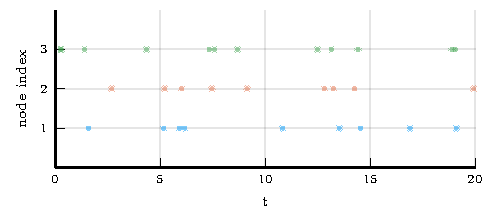
\includegraphics{assets/hawkes-barcode.pdf}}
\hfil
\subfloat[]{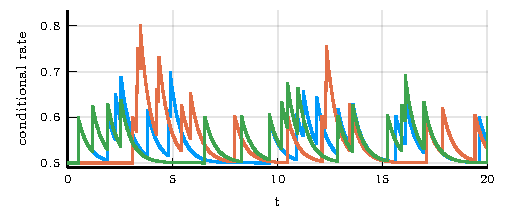
\includegraphics{assets/hawkes-intensity.pdf}}
\hfil
\subfloat[]{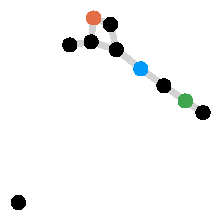
\includegraphics[width=113pt]{assets/mediumG.pdf}}
\subfloat[]{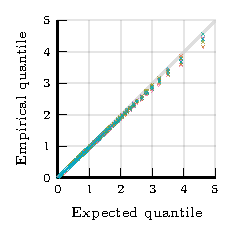
\includegraphics{assets/hawkes-qqplot.pdf}}
\caption{Simulations of 10-nodes compound Hawkes process with parameters \( \lambda = 0.5 , \alpha = 0.1 , \beta = 2.0 \) for \( 200 \) units of time. (a) and (b) sampled trajectory and intensity rate for a single simulation for the three selected nodes in (c) for the first \( 20 \) units of time. (c) underlying 10-nodes network with three random nodes selected. (d) QQ-plot of transformed inter-event time for 250 simulations colored by node.}
\label{fig:hawkes}
\end{figure}

Next, we assess the speed of the different aggregators. \texttt{SciMLBenchmarks.jl} includes four jump benchmarks for point processes over the real line: a 1-dimensional continuous time random walk approximation of a diffusion model (Diffusion), the multi-state model from Appendix A.6~\cite{marchetti2017} (Multi-state), a simple negative feedback gene expression model (Gene I) and the negative feedback gene expression from~\cite{gupta2018} (Gene II). The intensity rate of all the modelled processes in these benchmarks are constant between jumps. We simulate a single trajectory for each aggregator to visually check that they produce similar trajectories for a given model. The Diffusion, Multi-state, Gene I and Gene II benchmarks are then simulated \( 50 \), \( 100 \), \( 2000 \) and \( 200 \) times, respectively. Check the source code for further implementation details. Benchmark results are listed in Table~\ref{tab:benchmark-biochemistry}. The table shows that no single aggregator dominates suggesting they should be selected according to the task at hand. We also note that the performance of \texttt{Coevolve} matches \texttt{NRM} except for the last problem. Further investigation is needed to understand this difference in performance since the former should reduce to the latter when no \texttt{VariableRateJump} is used.

\begin{table}
\centering
\begin{tabular}{lccccc}
\toprule
\textbf{ Benchmark } & \multicolumn{1}{c}{\textbf{ Diffusion }} & \multicolumn{1}{c}{\textbf{ Multi-state }} & \multicolumn{1}{c}{\textbf{ Gene I }} & \multicolumn{1}{c}{\textbf{ Gene II }} \\
\texttt{Direct} & 4.85 s & 0.12 s & 0.17 ms & 0.44 s \\
\texttt{FRM} & 15.88 s & 0.22 s & 0.24 ms & 0.62 s \\
\texttt{SortingDirect} & 1.17 s & 0.12 s & 0.21 ms & 0.39 s \\
\texttt{NRM} & 0.87 s & 0.27 s & 0.44 ms & 0.75 s \\
\texttt{DirectCR} & 0.43 s & 0.20 s & 0.38 ms & 0.79 s \\
\texttt{RSSA} & 1.91 s & 0.11 s & 0.35 ms & 0.59 s \\
\texttt{RSSACR} & 0.37 s & 0.16 s & 0.73 ms & 0.83 s \\
\texttt{Coevolve} & 0.77 s & 0.28 s & 0.40 ms & 0.96 s \\
\bottomrule
\end{tabular}
\caption{Median execution time. A 1-dimensional continuous time random walk approximation of a diffusion model (Diffusion), the multi-state model from Appendix A.6~\cite{marchetti2017} (Multi-state), a simple negative feedback gene expression model (Gene I) and the negative feedback gene expression from~\cite{gupta2018} (Gene II).}
\label{tab:benchmark-biochemistry}
\end{table}

Finally, we add a new benchmark to the benchmark suite which simulates the compound Hawkes process for an increasing number of self-exciting processes. Let a graph with \( V \) nodes, then the compound Hawkes process is characterized by \( V \) point processes such that the conditional intensity rate of node \( i \) connected to a set of nodes \( E_i \) in the graph is given by
\[
  \lambda_i^\ast (t) = \lambda + \sum_{j \in E_i} \sum_{t_{n_j} < t} \alpha \exp \left[-\beta (t - t_{n_j}) \right]
\]
This process is known as self-exciting, because the occurence of an event \( j \) at \( t_{n_j} \) will increase the conditional intensity of all the processes connected to it by \( \alpha \). The excited intensity then decreases at a rate proportional to \( \beta \).
\[
\begin{split}
  \frac{d \lambda_i^\ast (t)}{d t} 
    &= -\beta \sum_{j \in E_i} \sum_{t_{n_j} < t} \alpha \exp \left[-\beta (t - t_{n_j}) \right] \\
    &= -\beta \left( \lambda_i^\ast (t) - \lambda \right)
\end{split}
\]

The conditional intensity of this process has a recursive formulation which can significantly speed the simulation. The recursive formulation for the univariate case is derived in~\cite{laub2021}. We derive the compound case here. Let \( t_{N_i} = \max \{ t_{n_j} < t \mid j \in E_i \} \) and \( \phi_i^\ast (t) \) below.
\[
\begin{split}
  \phi_i^\ast (t) 
    % &= \sum_{j \in E_i} \sum_{t_{n_j} < t} \alpha \exp \left[-\beta (t - t_{n_j}) \right] \\
    &= \sum_{j \in E_i} \sum_{t_{n_j} < t} \alpha \exp \left[-\beta (t - t_{N_i} + t_{N_i} - t_{n_j}) \right] \\
    &= \exp \left[ -\beta (t - t_{N_i}) \right] \sum_{j \in E_i} \sum_{t_{n_j} \leq t_{N_i}} \alpha \exp \left[-\beta (t_{N_i} - t_{n_j}) \right] \\
    % &= \exp \left[ -\beta (t - t_{N_i}) \right] \left( \alpha + \sum_{j \in E_i} \sum_{t_{n_j} < t_{N_i}} \alpha \exp \left[-\beta (t_{N_i} - t_{n_j}) \right] \right) \\
    &= \exp \left[ -\beta (t - t_{N_i}) \right] \left( \alpha + \phi^\ast (t_{N_i}) \right)
\end{split}
\]
Then the conditional intensity can be re-written in terms of \( \phi_i^\ast (t_{N_i}) \)
\[
  \lambda_i^\ast (t) = \lambda + \phi_i^\ast (t) = \lambda + \exp \left[ -\beta (t - t_{N_i}) \right] \left( \alpha + \phi_i^\ast (t_{N_i}) \right)
\]

A random graph is sampled from the Erd\H{o}s-Rényi model. This model assumes the probability of an edge between two nodes is independent of other edges, which we fix at \( 0.2 \). Note that this setup implies an increasing expected node degree. 

We fix the Hawkes parameters at \( \lambda = 0.5 , \alpha = 0.1 , \beta = 5.0 \) ensuring the process does not explode and simulate models in the range from \( 1 \) to \( 95 \) nodes for \( 25 \) units of time. We simulate \( 50 \) trajectories with a limit of ten seconds to complete execution. 

We assess the benchmark in five different settings. First, we run the \textit{inverse} method and \texttt{Coevolve} using the brute force implementation of the intensity rate which loops through the whole history of past events. Second, we implement a recursive algorithm for computing the intensity rate which we use to run both methods. We also run the benchmark against \texttt{PiecewiseDeterministicMarkovProcesses.jl}~\footnote{\url{https://github.com/rveltz/PiecewiseDeterministicMarkovProcesses.jl}} which is developed by the same author who proposed the \textit{CHV} algorithm discussed in Subsection~\ref{subsec:sim-inverse}. Finally, we run the benchmark using the Python library Tick~\footnote{\url{https://github.com/X-DataInitiative/tick}}. This library implements a version of the thinning method for simulating the process and implements a recursive algorithm for computing the intensity rate. 

Table~\ref{tab:benchmark-hawkes} shows that \texttt{Coevolve} is orders of magnitude faster than the \textit{inverse} method for any system size. As shown in Algorithm~\ref{algo:sim-queueing}, every sampled point in \texttt{Coevolve} requires a number of expected updates equal to the expected degree of the dependency graph. Therefore, it is able to complete non-exploding simulations efficiently. Instead, the \textit{inverse} method is unable to complete within the allocated time for larger systems because it is required to find an ever larger number of roots of an ever larger system of differential equations. 

The recursive implementation of the intensity rate also brings considerable performance boost placing \texttt{Coevolve} as one of the fastest algorithms. The Python library \texttt{Tick} remains competitive for smaller problems, but gets considerably slower for bigger ones. Also, it is only specialized to the Hawkes process. Another drawback is that the library wraps the actual \texttt{C++} implementation. In contrast, \texttt{JumpProcesses.jl} can simulate many other point processes with a relatively simple user-interface provided by the Julia language. Finally, \textit{CHV} is slower for smaller networks, but slightly faster than \texttt{Coevolve} for larger models. The fact that \textit{CHV} is not well-integrated with the SciML organization might pose a challenge for some users.


\begin{table*}
\centering
\begin{tabular}{lccccllllllll} 
\toprule
 & \multicolumn{4}{c}{\textbf{ Brute force }} & \multicolumn{8}{c}{\textbf{Recursive}} \\
\textbf{ V } & \multicolumn{2}{c}{\textbf{ \textit{Inverse} }} & \multicolumn{2}{c}{\textbf{\texttt{ Coevolve }}} & \multicolumn{2}{c}{\textbf{ \textit{Inverse} }} & \multicolumn{2}{c}{\textbf{\texttt{ Coevolve }}} & \multicolumn{2}{c}{\textbf{\textit{ CHV }}} & \multicolumn{2}{c}{\textbf{ \texttt{Tick} }} \\
            & n  & time              & n  & time              & n  & time              & n  & time                            & n  & time                          & n             & time              \\
\textbf{1}  & 50 & 143.4 \( \mu s \) & 50 & 2.6 \( \mu s \)   & 50 & 104.3 \( \mu s \) & 50 & \textbf{4.1} \( \bm{\mu s} \)   & 50 & \underline{150.0 \( \mu s \)} & 50            & 28.3 \( \mu s \)  \\
\textbf{10} & 50 & 16.0 ms           & 50 & 342.0 \( \mu s \) & 50 & 9.8 ms            & 50 & \textbf{96.0} \( \bm{\mu s} \)  & 50 & \underline{472.2 \( \mu s \)} & 50            & 134.6 \( \mu s \) \\
\textbf{20} & 50 & 106.8 ms          & 50 & 2.5 ms            & 50 & 47.0 ms           & 50 & \textbf{356.1} \( \bm{\mu s} \) & 50 & \underline{713.3 \( \mu s \)} & 50            & 933.5 \( \mu s \) \\
\textbf{30} & 29 & 344.8 ms          & 50 & 5.7 ms            & 50 & 158.0 ms          & 50 & \textbf{649.2} \( \bm{\mu s} \) & 50 & \underline{1.2 ms}            & 50            & 3.0 ms            \\
\textbf{40} & 6  & 1.9 s             & 50 & 13.6 ms           & 9  & 1.2 s             & 50 & \textbf{1.2 ms}                 & 50 & \underline{1.4 ms}            & 50            & 7.3 ms            \\
\textbf{50} & 3  & 3.6 s             & 50 & 26.0 ms           & 5  & 2.4 s             & 50 & \textbf{1.8 ms}                 & 50 & \underline{1.8 ms}            & 50            & 14.3 ms           \\
\textbf{60} & 2  & 6.9 s             & 50 & 45.6 ms           & 3  & 4.3 s             & 50 & \underline{2.5 ms}              & 50 & \textbf{2.5  ms}              & 50            & 28.9 ms           \\
\textbf{70} & 2  & 9.5 s             & 50 & 72.3 ms           & 2  & 6.6 s             & 50 & \underline{3.5 ms}              & 50 & \textbf{2.9 ms}               & 50            & 56.9 ms           \\
\textbf{80} & 1  & 15.4 s            & 50 & 118.7 ms          & 1  & 10.9 s            & 50 & \underline{4.3 ms}              & 50 & \textbf{3.5 ms}               & 50            & 97.8 ms           \\
\textbf{90} & 1  & 26.0 s            & 50 & 146.3 ms          & 1  & 17.4 s            & 50 & \underline{5.3 ms}              & 50 & \textbf{4.4 ms}               & 50            & 160.8 ms          \\
\bottomrule
\end{tabular}
\caption{Median execution time for the compound Hawkes process, V is the number of nodes and n is the total number of successful executions under ten seconds. Brute force refers to the implementation of the intensity rate looping through the whole history of past events. Recursive refers to a recursive implementation that only requires looking at the previous state of each node. \textit{Inverse} and \texttt{Coevolve} are algorithms from \texttt{JumpProcesses.jl}, \textit{CHV} is an algorithm from \texttt{PiecewiseDeterministicMarkovProcesses.jl} and \texttt{Tick} is a Python library. Fastest time is \textbf{bolded}, second fastest \underline{underlined}.}
\label{tab:benchmark-hawkes}
\end{table*}

\section{Conclusion}

This paper demonstrates that \texttt{JumpProcesses.jl} is a fast, general-purpose library for simulating evolutionary point processes. With the addition of the \texttt{Coevolve} aggregator, any point process on the real line with a non-negative, left-continuous, history-adapted and locally bounded intensity rate can be simulated with this library. The objective of this paper was to bridge the gap between the treatment of point process simulation in statistics and biochemistry. We demonstrated that many of the algorithms developed in biochemistry which served as the basis for the \texttt{JumpProcesses.jl} aggregators can be mapped to three general methods developed in statistics for simulating evolutionary point processes. We showed that the existing aggregators mainly differ in how they update and sample from the intensity rate and mark distribution. As we performed this exercise, we noticed the lack of an efficient aggregator for variable intensity rates in \texttt{JumpProcesses.jl}, a gap which \texttt{Coevolve} is meant to fill.

\texttt{Coevolve} borrows many enhacements from other aggregators in \texttt{JumpProcesses.jl}. However, there are still a number of ways forward. First, the aggregator cannot simulate processes whose rate depends on variables from differential equations. This extension would allow two-way interoperability with the rest of the SciML family. Next, we should consider whether it is possible to reduce the number of iterations during thinning. Processes get updated once its dependencies change. Once we know a process will not fire before one of its dependencies, we should be able to stop the iteration and wait for the update or continue from where the iteration stopped if the dependency gets delayed. This might become important once we allow rates that depend on differential equations. Third, given the performance of the \textit{CHV} algorithm in our benchmarks, we should consider adding it to \texttt{JumpProcesses.jl} as another aggregator such that it can benefit with tighter integration with the SciML organization. Fourth, \texttt{JumpProcesses.jl} would benefit from further development in inexact methods. At the moment, support is limited to processes with constant rates between jumps and does not support marks. Inexact methods should allow for the simulation of longer periods of time when only an event count per time interval is required. Hawkes processes can be expressed as a branching process. There are simulation algorithms that already take advantage of this structure to leap through time~\cite{laub2021}. It would be important to adapt these algorithms for general, compound branching processes to cater for a larger number of settings. Finally, \texttt{JumpProcesses.jl} also includes algorithms for jumps over two-dimensional spaces. It might be worth conducting a similar comparative exercise to identify algorithms in statistics for \(2 \)- and \( N \)-dimensional processes that could also be added to \texttt{JumpProcess.jl} as it has the potential to become the go-to library for general point process simulation.

\bibliographystyle{juliacon}
\bibliography{references}
\end{document}
